% !TEX root =  ../Dissertation.tex

\chapter{Results}
\label{ch:results}

This chapter reports the findings of the various experiments, in the order of the research questions. Throughout, a reported Sharpe ratio means the annualised excess Sharpe of the concatenated test stream, calculated from Eq. \ref{eq:sharpe}. Learned arms are the mean over the 5 seeds $\{0,\dots,4\}$ with the standard deviation across seeds. Baselines are deterministic and have no seed spread (except LSTM). Differences between arms are tested with the paired stationary bootstrap \cite{politis1994stationary} and the Ledoit-Wolf HAC Sharpe-difference test.

\section{What the regimes track}
\label{sec:results-interpretation}
RQ1 asks whether the regimes discovered by our method(rung 2) differ from statistically defined ones. To start, I choose $K=3$, which gives three gates for the three cases; I first plot them to get a visual understanding, particularly of how much they switch, as shown in Fig. \ref{fig:ribbons}. Then I compute the pairwise correlations among the three. For this, I did two things: first, I found the percentage of overlapping area between pairs, and second, I computed the AMI.

\begin{figure}[t]
  \centering
  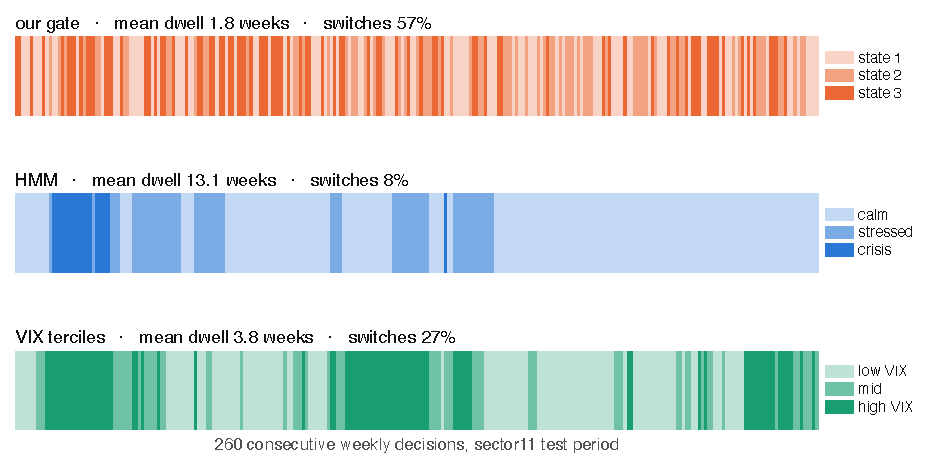
\includegraphics[width=\textwidth]{fig_regime_ribbons.pdf}
  \caption[Regime timelines]{Weekly regime labels over five consecutive years of the \texttt{sector11} test period. Over the full test period the mean dwell times are $1.8$, $12.9$ and $3.7$ weeks for the learned gate, HMM and VIX terciles; within the five-year window shown they are $1.8$, $13.1$ and $3.8$.}
  \label{fig:ribbons}
\end{figure}

\begin{figure}[t]
  \centering
  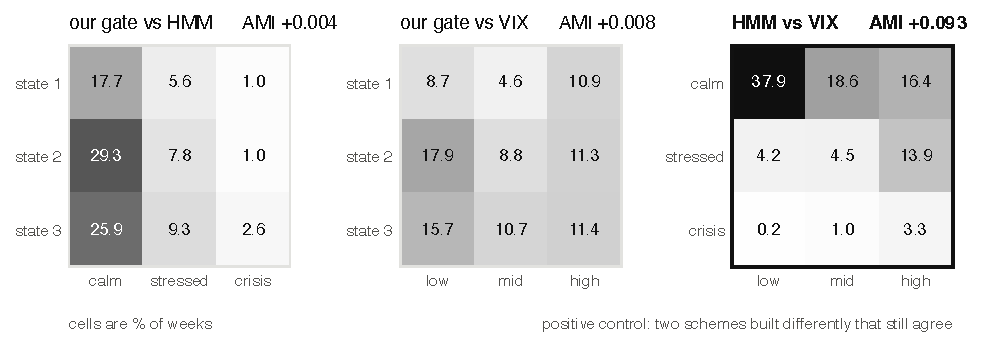
\includegraphics[width=\textwidth]{fig_regime_agreement.pdf}
  \caption[Regime agreement]{Co-occurrence of weekly regime labels on
  \texttt{sector11}, as a percentage of weeks, with the chance-corrected
  agreement (AMI) above each panel.}
  \label{fig:agreement}
\end{figure}

\paragraph{The partitions are effectively orthogonal.}
The key finding is from Fig. \ref{fig:agreement} on \texttt{sector11} the learned gate agrees with the HMM at AMI $+0.004$ and with the VIX terciles at $+0.008$; on \texttt{etf10} the values are $-0.002$ and $+0.020$. These are very small values and likely just by chance. However between the HMM and the VIX gate agree with each other at $+0.093$ on \texttt{sector11}, an order of magnitude above either of their agreements with the learned gate. On \texttt{etf10} the control pairing is weaker ($+0.017$), so the sub-claim that the two statistical schemes cluster together holds only on \texttt{sector11}.

This can also be observed visually from Fig. \ref{fig:agreement} , if we see the chart, if two methods were correlated then that means knowing which regime lead in one tells significant information of which regime leads in other. So we say take a column then one of this row should have significantly larger values then the others. This is only seen in the third chart, thus the two statistical gates have more in common with each other then with our gate.

\begin{figure}[t]
  \centering
  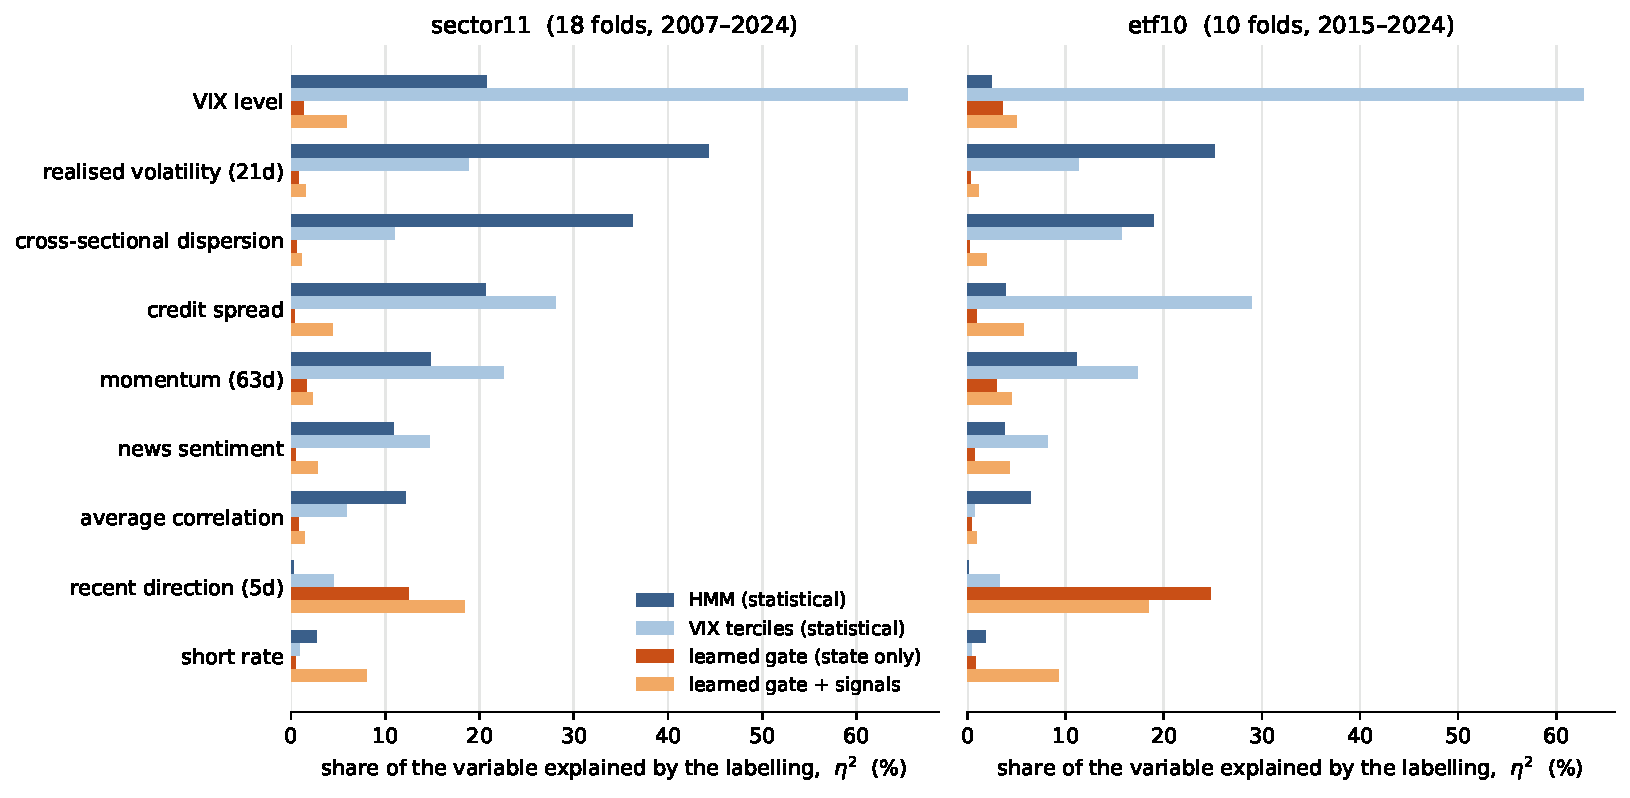
\includegraphics[width=\textwidth]{fig_gate_with_signals.pdf}
  \caption[What each regime scheme tracks]{The share of each market variable explained by each labelling.  The light orange bars are the same gate re-trained with all five market-level signals of Section~\ref{sec:signals} appended to its input: direction remains its leading variable and realised volatility stays at the floor. The figure labels abbreviate the five-signal vector as ``signals''.}
  \label{fig:eta2}
\end{figure}

\paragraph{Each scheme measures a different quantity.}
Using the method described in \ref{sec:baselines}, I estimate the underlying significance value for each of the three ways I generate the gates. From this, we see that the statistical gates are risk detectors: the HMM labeling explains $44.3\%$ of trailing realized volatility on \texttt{sector11} ($25.2\%$ on \texttt{etf10}), and the VIX gate explains $65.4\%$ of its own index. For our gate, the best explanation appears to be that it is a direction detector, since its leading variable is the trailing five-day return, at $12.5\%$ on \texttt{sector11} and $24.8\%$ on \texttt{etf10}. At the same time, it explains under $1\%$ of realized volatility. 

\paragraph{Equal information: adding market signals as well.}
The comparison so far is open to one objection: the statistical gates read market observables, while the learned gate reads only the reservoir state, so perhaps it tracks direction because it never saw a risk variable. The light-orange bars in Figure~\ref{fig:eta2} close this. The same mixture is re-trained with the five market-level signals, VIX included, concatenated to the gate's input (the routing of Section~\ref{sec:gate}). We see the gate using the new labelling because its AMI with preceding state only gate is  $0.165$--$0.180$ rather than $1$. The metric with the largest change is the short rate whose $\eta^2$ rises by around $8\%$. But it does not reorganise with respect to risk. Recent direction remains its leading variable ($18.4\%$ on both universes), realised volatility stays at the floor ($1.6\%$ and $1.1\%$, still roughly twenty-five times below the HMM). Even agreement with the statistical gates stays at chance (AMI $\le 0.022$).

\section{The walk-forward ladder}
\label{sec:results-ladder}

RQ2 asks whether the carving pays. Table~\ref{tab:ladder} and Figure~\ref{fig:ladder} report every arm on the full walk-forward test span: eighteen folds on \texttt{sector11} (test years 2007-2024, 4530 trading
days) and ten on \texttt{etf10} (2015-2024, 2516 days).

\begin{table}[t]
  \centering
  \small
  \begin{tabular}{l rrr rrr}
    \hline
    & \multicolumn{3}{c}{\texttt{sector11} (2007--24)}
    & \multicolumn{3}{c}{\texttt{etf10} (2015--24)} \\
    arm & Sharpe & turn & maxDD & Sharpe & turn & maxDD \\
    \hline
    1/N                      & 0.485 & 1.3 & $-53\%$ & 0.374 & 1.3 & $-23\%$ \\
    buy-and-hold SPY         & 0.510 & 1.0 & $-55\%$ & \textbf{0.688} & 1.0 & $-34\%$ \\
    inverse-volatility       & 0.511 & 1.7 & $-50\%$ & 0.278 & 1.8 & $-21\%$ \\
    Ledoit--Wolf MV          & 0.479 & 4.5 & $-35\%$ & 0.058 & 4.4 & $-38\%$ \\
    \hline
    ours, $K{=}1^{\dagger}$            & 0.414 $\pm$ 0.019 & 12.5 & $-51\%$ & 0.296 $\pm$ 0.028 & 8.4 & $-23\%$ \\
    ours, $K{=}3^{\ddagger}$           & 0.461 $\pm$ 0.030 & 10.3 & $-49\%$ & 0.237 $\pm$ 0.025 & 8.1 & $-23\%$ \\
    3a signals $\to$ gate    & 0.488 $\pm$ 0.045 &  9.5 & $-50\%$ & 0.280 $\pm$ 0.057 & 7.5 & $-23\%$ \\
    3b signals $\to$ experts & 0.469 $\pm$ 0.063 &  8.8 & $-47\%$ & 0.272 $\pm$ 0.036 & 9.4 & $-23\%$ \\
    3c signals $\to$ both    & 0.500 $\pm$ 0.043 &  9.6 & $-44\%$ & 0.264 $\pm$ 0.017 & 7.5 & $-23\%$ \\
    ours, $K{=}1$ + signals  & 0.507 $\pm$ 0.027 &  9.8 & $-49\%$ & 0.318 $\pm$ 0.034 & 8.1 & $-22\%$ \\
    \hline
    HMM gate                 & 0.418 $\pm$ 0.015 & 11.7 & $-47\%$ & 0.312 $\pm$ 0.020 & 10.6 & $-20\%$ \\
    VIX gate                 & 0.408 $\pm$ 0.036 & 12.4 & $-52\%$ & 0.232 $\pm$ 0.022 & 11.4 & $-29\%$ \\
    LSTM (trained encoder)   & 0.378 $\pm$ 0.017 &  4.0 & $-50\%$ & 0.299 $\pm$ 0.027 & 4.4 & $-19\%$ \\
    \hline
    \multicolumn{7}{l}{\emph{shown for reference only; values with best found K}}\\
    best capacity$^{\S}$ ($K{=}2$ / $K{=}5$)
                             & \textbf{0.513} $\pm$ 0.025 & --- & --- & 0.408 $\pm$ 0.106 & --- & --- \\
    \hline
  \end{tabular}
  \caption[The walk-forward ladder]{Concatenated test Sharpe (mean $\pm$
  standard deviation over five head seeds), annualised one-way turnover and
  maximum drawdown. The best value in each Sharpe column is in
  bold. $\dagger$\,frozen configuration on \texttt{sector11};
  $\ddagger$\,frozen configuration on \texttt{etf10}
  (Table~\ref{tab:hyper}). ``Signals'' is the five-signal vector of
  Section~\ref{sec:signals}.
  (Section~\ref{sec:results-capacity}).}
  \label{tab:ladder}
\end{table}
\begin{figure}[t]
  \centering
  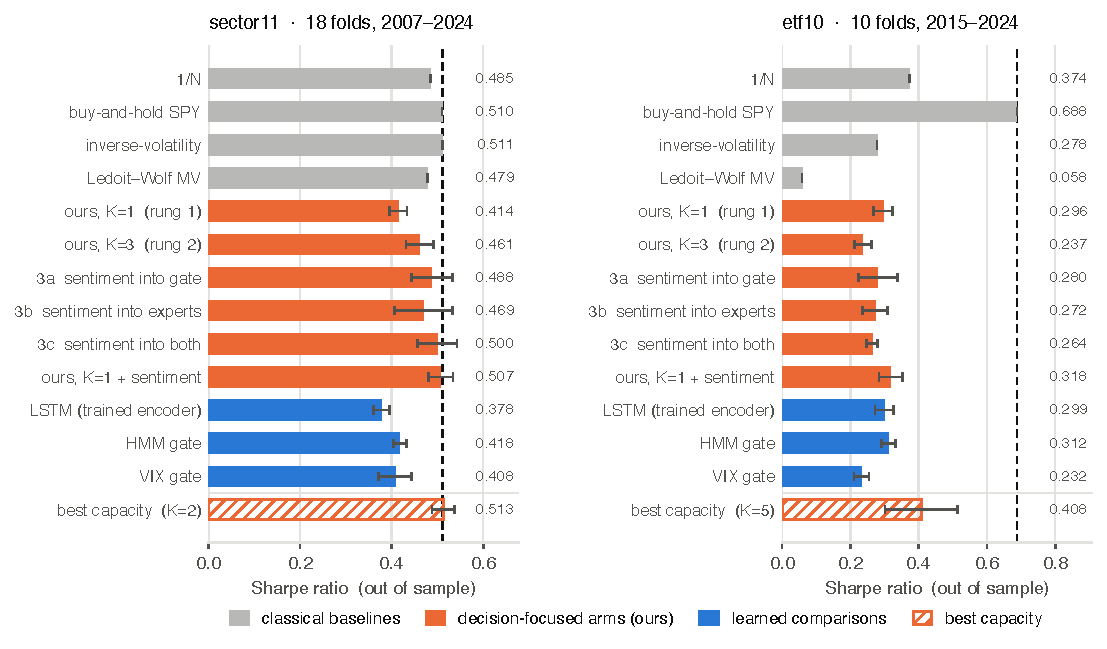
\includegraphics[width=\textwidth]{fig_ladder_sharpe.pdf}
  \caption[Ladder comparison]{The ladder of Table~\ref{tab:ladder}. Error bars
  are seed dispersion, not significance intervals; the baselines are
  deterministic and show none. The dashed line marks the best baseline in each
  universe. The ``rung'' numbers in the labels index the build order of the
  study, and ``sentiment'' in the arm labels abbreviates the five-signal
  vector.}
  \label{fig:ladder}
\end{figure}

No learned arm beats the best baseline on either universe. On \texttt{sector11} the best learned arm is the single head with the signals appended ($0.507 \pm 0.027$), ties the inverse-volatility baseline ($0.511$) while trading nearly six times as much. On \texttt{etf10} it is not close: SPY scores $0.688$ and the best learned arm $0.318$. The two statistical gates do no better ($0.418$ and $0.408$ on \texttt{sector11}; $0.312$ and $0.232$ on \texttt{etf10}), so the null is not specific to how the regimes are formed: conditioning on regimes, however defined, did not pay here i.e. none of the learned differences is significant. Each arm is compared with its neighbor on the ladder, the net difference in max and min of ours is only about 0.1.
\begin{figure}[t]
  \centering
  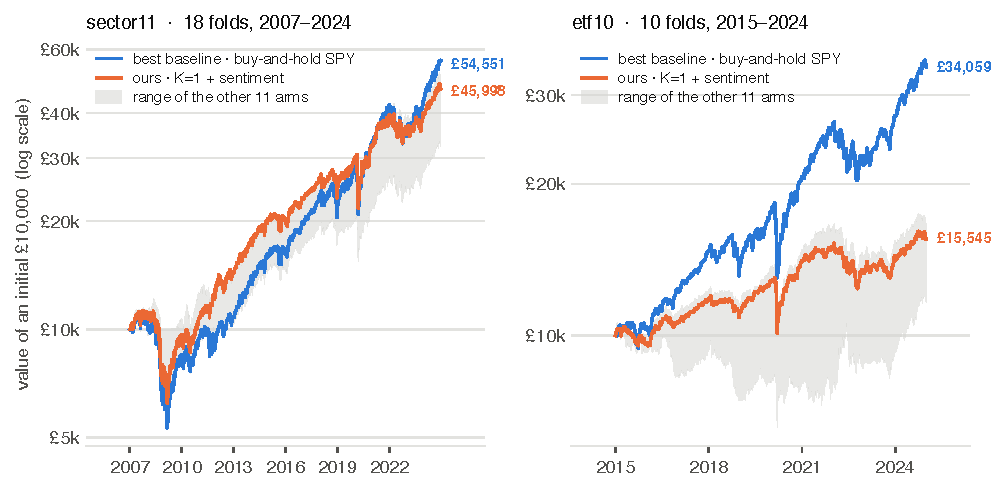
\includegraphics[width=\textwidth]{fig_growth_10k.pdf}
  \caption[Growth of \pounds10{,}000]{Growth of an initial \pounds10{,}000, using the seed-0 stream of the best learned arm against the best baseline; the grey band is the min--max envelope of the other eleven arms.}
  \label{fig:growth}
\end{figure}

On account of money gained, the seed-0 stream of the best learned arm turns \pounds10{,}000 into \pounds45{,}998 on \texttt{sector11} against \pounds54{,}551 for buy-and-hold SPY, and into \pounds15{,}545 on \texttt{etf10} against \pounds34{,}059 (Figure~\ref{fig:growth}). From the figure two interesting things are seen. First, on \texttt{sector11} the learned arm is ahead of SPY for most of a decade and the lead changes only after 2021. I do not read this as a regime the model exploited and then lost rather for such wide intervals one path crossing another for years at a time is what a tie looks like. Second, in 2008 the learned arm rides the crash down with the market, losing roughly half its value; its drawdown ($-49\%$) is close to SPY's ($-55\%$). Meaning the gating detects nothing that would have removed it from harm's way, which is consistent with Section~\ref{sec:results-interpretation}: a direction detector reacts to a crash once prices have already fallen.

\paragraph{Additional context to the results of \texttt{etf10} }
On \texttt{etf10} every diversified allocation lost to SPY over 2015-2024: 1/N scores $0.374$, inverse-volatility $0.278$ and Ledoit--Wolf mean-variance $0.058$, because bonds fell as rates rose and non-US equity and commodities lagged US large-caps for the whole decade. The learned arms sit beside 1/N, which is what they learned to be. The honest reading is not that the model is uniquely broken on \texttt{etf10} but that diversification itself lost to the index in that window, and the model paid the same price plus turnover.

\section{Capacity, selection and transfer}
\label{sec:results-capacity}

RQ3 asks whether more capacity or more information helps: more experts, a trained encoder(LSTM) in place of the frozen reservoir, extra signals. The signal part was answered negatively above. This section reports impact of the other two.

\begin{figure}[t]
  \centering
  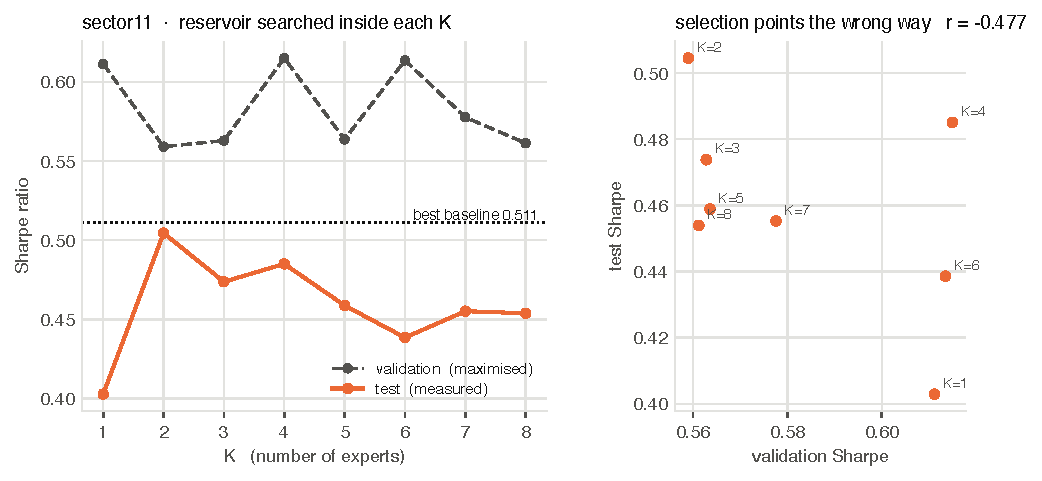
\includegraphics[width=\textwidth]{fig_capacity_curve.pdf}
  \caption[Capacity curve]{Left: validation and test Sharpe against the number of experts $K$ on \texttt{sector11}, with the reservoir searched inside each $K$ and the winner scored on the full walk-forward test. Right: the same eight points as a scatter, validation and test anti-correlate ($r=-0.477$)(Section~\ref{sec:results-capacity}).}
  \label{fig:capacity}
\end{figure}

\paragraph{Impact of more experts.}
Figure~\ref{fig:capacity} gives each $K \in \{1,\dots,8\}$ its own small reservoir hyperparameter search and scores each winner on the full test span. On \texttt{sector11}, $K=1$ is the worst capacity on test ($0.403$) and $K=2$ the best ($0.505$); $K=2$, $5$, $7$ and $8$ all resolve above $K=1$ by more than two seed spreads. The searched reservoir width also grows with $K$ (from $300$ to $600$ units).


\paragraph{Selection on validation points the wrong way.}
The right panel of Figure~\ref{fig:capacity} is the sharpest result in this chapter. Across the eight capacities, validation and test Sharpe have negative correlation at $r=-0.477$: $K=4$ has the best validation score of all eight and lands mid-table on test, while $K=2$ has nearly the worst validation and the best test. On \texttt{etf10} the correlation is positive ($r=+0.678$), so the anti-correlation is a \texttt{sector11} finding and not a law.

\begin{table}[t]
  \centering
  \small
  \begin{tabular}{lll rrr}
    \hline
    search & universe & encoder & selection & held out & untuned ref.\\
    \hline
    grid, $N_r\times\rho$ & \texttt{sector11} & reservoir & 0.603 $\pm$ 0.02 & 0.526 $\pm$ 0.09 & 0.534 $\pm$ 0.02 \\
    joint, $K\times\rho$  & \texttt{sector11} & reservoir & 0.582 & 0.428 & 0.509 \\
    random, 50 draws      & \texttt{etf10}    & reservoir & 0.438 $\pm$ 0.07 & 0.929 $\pm$ 0.15 & 0.811 $\pm$ 0.05 \\
    joint, $K\times\rho$  & \texttt{etf10}    & reservoir & 0.464 & 0.783 & 0.809 \\
    staged, 16+ cells     & \texttt{sector11} & LSTM      & 1.011 & 0.738 $\pm$ 0.22 & 0.554 $\pm$ 0.04 \\
    staged, 16+ cells     & \texttt{etf10}    & LSTM      & 1.068 & 0.473 $\pm$ 0.04 & 0.605 $\pm$ 0.06 \\
    \hline
  \end{tabular}
  \caption[Held-out verification of searched winners]{Every configuration
  selected by a search, re-scored on folds excluded from all selection
  (\texttt{sector11} F13--F18, \texttt{etf10} F06--F10). ``Selection'' is the
  winner's score on the folds it was selected on; ``held out'' its score on
  the excluded folds; ``untuned ref.''\ the untouched reference on the same
  held-out folds (the Appendix-B reservoir defaults, or for the LSTM the
  fixed ladder configuration). Values without a spread are single re-scored
  runs.}
  \label{tab:transfer}
\end{table}

\paragraph{No searched winner transferred.}
Table~\ref{tab:transfer} re-scores every searched winner on folds that took no part in any selection. On \texttt{sector11} both reservoir winners come back at or below the untuned defaults, one of them badly ($0.582$ on its selection folds, $0.428$ held out, against the defaults' $0.509$). On \texttt{etf10} the random-search winner comes back $0.118$ ahead of the defaults, inside one seed spread ($0.150$), which is no evidence of transfer rather than evidence of failure; the joint winner comes back slightly behind. The two LSTM champions are the largest reversals: validation scores of $1.011$ and $1.068$ collapse to $0.738$ and $0.473$ held out, the latter below even the untuned ladder configuration.

\begin{figure}[t]
  \centering
  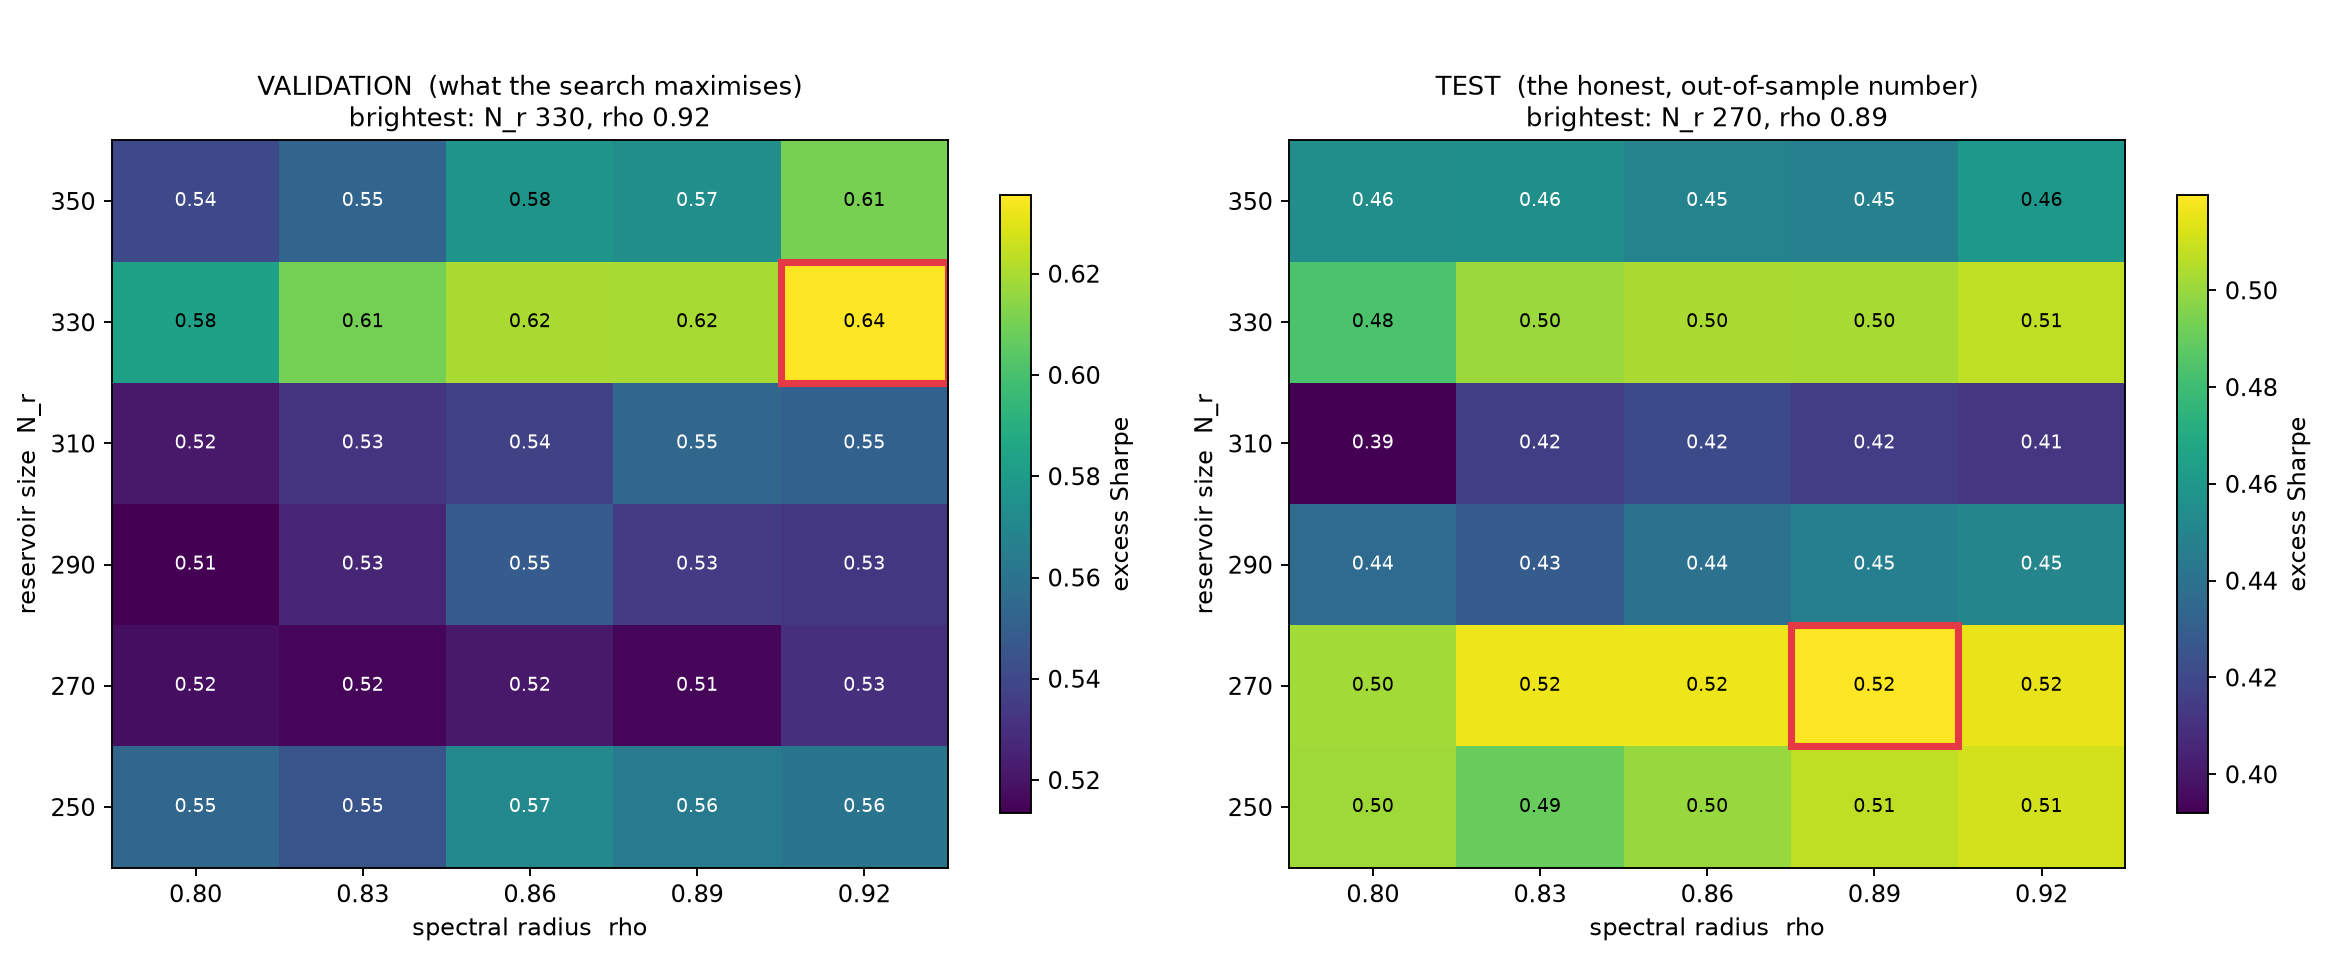
\includegraphics[width=\textwidth]{fig_grid_val_vs_test.png}
  \caption[Validation against test on the fine grid]{The $N_r \times \rho$
  slice of the fine grid at default parameters, \texttt{sector11},
  $K=2$: validation Sharpe (left) and test Sharpe (right) on the same cells,
  each panel's best cell boxed. The maximum do not coincide, and the
  validation best row ($N_r=330$) is mediocre on test while the
  validation worst row ($N_r=270$) is the test-hottest.}
  \label{fig:heatmap}
\end{figure}

\paragraph{A dense grid finds nothing to fix.}
A final, denser search was performed with $1{,}485$ configurations in a local grid around each universe's best values ($810$ on \texttt{sector11}, $675$ on \texttt{etf10}), validated on the selection folds, with the top twelve re-scored on the full test span.  Neither winner survived the move. On \texttt{sector11} the best cell on validation scored $0.678$ there and $0.522$ on test, against the $0.505$ the configuration already in hand reached. The highest test score among the twelve was $0.532$, but that is the largest of twelve noisy numbers, and a single number here moves by $0.02$ to $0.06$ on the choice of seed alone, so it is not meaningfully better. On \texttt{etf10} the gap is wider: the validation winner scored $0.659$ and then tested at $0.250$, well below the $0.411$ already in hand, which remained the best test score found anywhere in the grid.

So searching harder only lifted the validation ceiling, from $0.559$ to $0.678$. The test scores did not follow it up. Figure~\ref{fig:heatmap} shows why by showcasing that for one slice of the grid the settings that do well on validation and the settings that do well on test are not the same settings. 

\paragraph{The trained encoder.}
Till now I gave the LSTM one hand-picked configuration while the reservoir side had run hundreds of search trials, so the comparison was not yet fair. A matched search fixes this. Here the size of hidden state and lookback matters. When we increase hidden states from $16 \to 128$ it raises validation Sharpe by $0.456$ on \texttt{sector11} and $0.347$ on \texttt{etf10}. The impact of lookback is much lower, increasing it from $20 \to 250$ moves it by at most $0.067$. So the $60$-day window was never the handicap, which the reservoir's own memory capacity corroborates. But that capacity bought validation score that did not last. Both champions fall from $1.011$ and $1.068$ to $0.738$ and $0.473$ on the folds held out of the search (Table~\ref{tab:transfer}), and on the ladder's own metric they reach only $0.237$ and $0.254$ where the pre-specified configuration reaches $0.378$ and $0.299$.


\paragraph{Effect of regularisation.}
If the train validation gap was due to overfitting, a penalty function can be used to reduce it and improve performance. Five penalties were implemented and swept: CVaR, turnover, expert diversity, weight decay and drawdown. All five select to zero (Table~\ref{tab:penalty}). Weight decay is the penalty on larger weight, thus this should have best impact on closing the train validation gap from $0.84$ to $-0.11$, yet final validation still gets worse. Consistently, raising $K$ adds parameters and widens the gap (from $-0.006$ at $K=1$ to $+0.047$ at $K=6$) while train Sharpe does not improve at all ($0.482$, $0.476$, $0.462$ at $K=1,3,6$) meaning the extra capacity buys variance, not fit.
Chapter~\ref{ch:discussion} argues that this pattern, no penalty computed on
the training window helps, is what non-stationarity looks like, as opposed to
overfitting.

\begin{table}[t]
  \centering
  \small
  \begin{tabular}{l rrr}
    \hline
    penalty & $\lambda=0$ & small & large \\
    \hline
    $\lambda_{\text{cvar}}$ (1.0 / 5.0)   & \textbf{0.526} & 0.505 & 0.449 \\
    $\lambda_{\text{turn}}$ (0.5 / 2.0)   & \textbf{0.526} & 0.403 & 0.412 \\
    $\lambda_{\text{div}}$ (0.01 / 0.05)  & \textbf{0.547} & 0.526 & 0.443 \\
    \hline
  \end{tabular}
  \caption[Loss penalties select to zero]{Validation-era sweeps of the three
  loss penalties on \texttt{sector11} (concatenated metric; the two sweeps in
  the upper rows share a base configuration, the third ran at a slightly
  different one). Every penalty is best at zero. The turnover penalty cuts
  turnover from $9.2$ to $1.8$ and costs $0.12$ of Sharpe; weight decay and a
  drawdown penalty, swept separately, also select to zero.}
  \label{tab:penalty}
\end{table}


\section{The holdout}
\label{sec:results-holdout}

The final eighteen months, 2 January 2025 to 30 June 2026 ($373$ trading days, $78$ weekly decisions), were firewalled from the start of the project (Section~\ref{sec:universes}) and evaluated once, by a dedicated script. Since I found no transference and optimal hyperparameters I use the initial best found values as frozen defaults. Training data end in December 2023, and 2024 served as validation. Alongside the frozen primary ($K=1$ on \texttt{sector11}, $K=3$ on \texttt{etf10}, all defaults) I ran one searched secondary, the best-capacity winner of Section~\ref{sec:results-capacity}, to measure what selecting the searched configuration would do, and the four baselines.

\begin{table}[t]
  \centering
  \small
  \begin{tabular}{l rrr}
    \hline
    \texttt{sector11} & Sharpe & maxDD & turnover \\
    \hline
    1/N                                  & \textbf{0.812} & $-15.0\%$ & 1.1 \\
    frozen $K{=}1$ (primary)             & 0.811 $\pm$ 0.033 & $-13.7\%$ & 3.6 \\
    searched $K{=}2$ (secondary)         & 0.809 $\pm$ 0.022 & $-13.7\%$ & 2.9 \\
    buy-and-hold SPY                     & 0.786 & $-18.8\%$ & 0.7 \\
    Ledoit--Wolf MV                      & 0.777 & $-14.5\%$ & 5.7 \\
    inverse-volatility                   & 0.710 & $-14.4\%$ & 1.5 \\
    \hline
    \texttt{etf10} & & & \\
    \hline
    1/N                                  & \textbf{1.340} & $-8.9\%$  & 1.0 \\
    Ledoit--Wolf MV                      & 1.313 & $-19.5\%$ & 2.0 \\
    frozen $K{=}3$ (primary)             & 1.295 $\pm$ 0.023 & $-8.3\%$ & 3.0 \\
    inverse-volatility                   & 1.136 & $-6.7\%$  & 1.5 \\
    searched $K{=}5$ (secondary)         & 0.930 $\pm$ 0.583 & $-6.8\%$ & 14.6 \\
    buy-and-hold SPY                     & 0.786 & $-18.8\%$ & 0.7 \\
    \hline
  \end{tabular}
  \caption[The holdout evaluation]{The single holdout run, 2025-01-02 to 2026-06-30. SPY scores identically on the two universes because it is the same asset on the same days, thus this serves like an internal consistency check of the pipeline.}
  \label{tab:holdout}
\end{table}

On top we see 1/N on both universes, and our frozen configuration lands closely behind with $0.811$ against $0.812$ on \texttt{sector11} and $1.295$ against $1.340$ on \texttt{etf10}. Thus the learned system performs like a diversified baseline, no better and no worse. For a study whose main performance result is a null, this is the preferable outcome, the holdout confirms what we have discussed till now instead of contradicting it.

On \texttt{sector11} the searched configuration does no better than the frozen one ($0.809$ against $0.811$); on \texttt{etf10} it is worse and wildly unstable ($0.930 \pm 0.583$ across seeds, at a turnover of $14.6$). Had I put a searched winner forward as the primary, the holdout would have returned a worse and less reliable number. One small observation runs in the model's favour: on both universes the frozen arm's maximum drawdown is shallower than that of every baseline that matches or beats its Sharpe.